\documentclass[11pt]{article}
\usepackage[margin=2cm]{geometry}
\usepackage{amsmath,amssymb}
\usepackage{graphicx}
\usepackage{booktabs}
\usepackage{xcolor}
\usepackage{tikz}
\usetikzlibrary{arrows.meta,decorations.pathreplacing,calc,backgrounds}
\usepackage{standalone}
\usepackage{fancyvrb}
\usepackage[compact]{titlesec}
\titleformat*{\section}{\large\bfseries}
\usepackage[font=small]{caption}
\usepackage[colorlinks=true,linkcolor=blue!50!black,urlcolor=blue!50!black]{hyperref}

\definecolor{cblue}{HTML}{1976D2}
\definecolor{cred}{HTML}{E53935}
\definecolor{cpurple}{HTML}{5E35B1}
\definecolor{cgrey}{HTML}{757575}

\newcommand{\bu}{\mathbf{u}}
\newcommand{\code}[1]{\texttt{#1}}
\fvset{fontsize=\footnotesize,xleftmargin=1em}

% Built from this folder by
%
%     tectonic recurrence-search.tex
%
% after fig_counts.jl has drawn figures/counts.pdf and the scripts of examples/lorenz/ their figures.
% The diagrams are those of the README, read from assets/diagrams/.

\begin{document}
\begin{center}
{\Large The search for near recurrences}\\[3pt]
The mathematics of \code{NearRecurrences.jl}
\end{center}

\section{What a near recurrence is}
\label{sec:recurrence}

A simulation advances a state $\bu$ and is sampled every $\Delta s$, so that sample $k$ is $\bu_k = \bu((k - 1)\,\Delta s)$, $k = 1, 2, \dots$ The system may have symmetries $\mathcal{S}(s)$, isometries that commute with the flow, continuous or discrete, with $s$ the vector of their shifts. The distance of a start $\bu(t)$ and an end $\bu(t + T)$ is
\begin{equation}
d(t, T) = \min_{s} \frac{\|\mathcal{S}(s)\,\bu(t + T) - \bu(t)\|}{\|\bu(t)\|} .
\label{eq:distance}
\end{equation}
It is zero when the end is a shifted copy of the start, that is on a relative periodic orbit of period $T$ and shift $s$, and small when the trajectory passes near one. Figure~\ref{fig:recurrence} draws such a pass. A near recurrence is a pair of samples where $d$ is a local minimum over $(t, T)$ and lies below a threshold $d_p$. It is the first guess of a Newton search for the orbit, with the shifts that reach the minimum in \eqref{eq:distance}.

\begin{figure}[h]
\centering
\documentclass[border=6pt]{standalone}
\usepackage{amsmath,amssymb}
\usepackage{xcolor}
\usepackage{tikz}
\usetikzlibrary{arrows.meta,backgrounds}
\definecolor{cblue}{HTML}{1976D2}
\definecolor{cred}{HTML}{E53935}
\definecolor{cpurple}{HTML}{5E35B1}
\definecolor{cgrey}{HTML}{757575}
\tikzset{every picture/.append style={show background rectangle,
    background rectangle/.style={fill=white}, inner frame sep=4pt}}
\newcommand{\bu}{\mathbf{u}}
% A near recurrence: the trajectory leaves u(t) and comes back close to a shifted copy of it.
\begin{document}
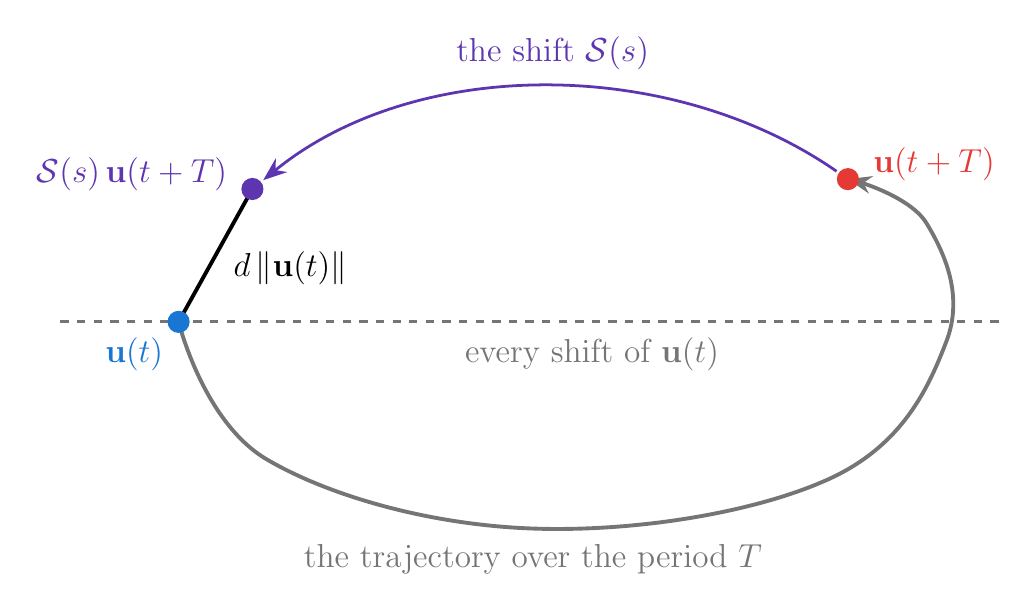
\begin{tikzpicture}[>={Stealth[length=3mm]}, every node/.style={font=\large}, x=1.25cm, y=1.25cm,
                    line width=1pt]
  % ---- the copies of the start under every shift ----
  \draw[cgrey, dashed] (-1.2, 0) -- (8.4, 0);
  \node[cgrey, below] at (4.2, -0.05) {every shift of $\bu(t)$};

  % ---- the trajectory over the period, below the copies and back above them ----
  \draw[cgrey, line width=1.4pt, ->] plot[smooth, tension=0.65] coordinates
      {(0, 0) (0.9, -1.4) (3.6, -2.1) (6.6, -1.6) (7.8, -0.2) (7.6, 1.0) (6.8, 1.45)};
  \node[cgrey, below] at (3.6, -2.15) {the trajectory over the period $T$};

  % ---- the start, the end, and the end shifted back near the start ----
  \draw[cpurple, ->, shorten >=5pt, shorten <=5pt] (6.8, 1.45) .. controls (5.0, 2.7) and (2.4, 2.7) .. (0.75, 1.35);
  \node[cpurple, above] at (3.8, 2.45) {the shift $\mathcal{S}(s)$};
  \draw[black, line width=1.4pt] (0, 0) -- (0.75, 1.35);
  \node[black, right] at (0.45, 0.55) {$d\,\|\bu(t)\|$};
  \fill[cblue] (0, 0) circle (4pt);
  \node[cblue, below left] at (-0.05, -0.05) {$\bu(t)$};
  \fill[cred] (6.8, 1.45) circle (4pt);
  \node[cred, right] at (6.95, 1.6) {$\bu(t + T)$};
  \fill[cpurple] (0.75, 1.35) circle (4pt);
  \node[cpurple, left] at (0.6, 1.5) {$\mathcal{S}(s)\,\bu(t + T)$};
\end{tikzpicture}
\end{document}

\caption{A near recurrence. The trajectory leaves $\bu(t)$ and after a time $T$ comes back close to a shifted copy of it. The shift that brings the end closest to the start leaves the distance $d$ of \eqref{eq:distance}, which a search reduces to zero.}
\label{fig:recurrence}
\end{figure}

The example of this note is Kolmogorov flow at $Re = 40$ with the forcing wavenumber $n_f = 4$, the vorticity advanced with the modes up to 33 on a grid of $100^2$ points by the scheme CB3R2R3e with steps $\Delta t = 0.01$, and sampled every $\Delta s = 0.1$, ten steps. It has two symmetries, the shift $\sigma$ along $x$, continuous, and the translations $s_y$ along $y$ by whole wavelengths of the forcing, discrete,
\begin{equation}
\mathcal{S}(\sigma, s_y)\,\omega(x, y) = \omega\big(x + \sigma,\ y + 2\pi s_y/n_f\big), \qquad \sigma \in [0, 2\pi),\quad s_y \in \{-1, 0, 1, 2\} .
\end{equation}
The norm is that of the vorticity, $\|\bu\|^2 = \sum_{jk} w_j |\hat\omega_{jk}|^2$, with $w_0 = 1$ and $w_j = 2$ for $j \ge 1$, since a mode $j \ge 1$ stands for its conjugate as well. The minimum over the shift and the translations follows Chandler \& Kerswell (2013, eq.~3.8), whose residual $R(t, T)$ is the square of such a distance, normalised by the later state instead of the earlier one, and whose pairs below a threshold are the guesses of Newton searches.

The minimum costs one pass over the coefficients. Since $\mathcal{S}$ is an isometry, for a start $a$ and an end $b$
\begin{equation}
\|\mathcal{S} b - a\|^2 = \|a\|^2 + \|b\|^2 - 2 f(\sigma, s_y), \qquad f(\sigma, s_y) = \mathrm{Re} \sum_{j=0}^{33} e^{\mathrm{i} j \sigma} \sum_{q=0}^{3} \mathrm{i}^{\,q s_y}\, G_{jq},
\label{eq:poly}
\end{equation}
with $G_{jq} = \sum_{k \equiv q\,(\mathrm{mod}\,4)} w_j\, \bar a_{jk} b_{jk}$, the sum over the wavenumbers $k$ along $y$. The shift multiplies $b_{jk}$ by $e^{\mathrm{i} j \sigma}$ and the translation by $\mathrm{i}^{\,k s_y}$, which depends on $k$ modulo 4 alone, so the products $\bar a_{jk} b_{jk}$ enter through the four sums $G_{jq}$. For each $s_y$, $f$ is then a trigonometric polynomial of degree 33 in $\sigma$. One inverse FFT of length 256 gives it at 256 shifts, and four Newton steps refine the largest value. A distance takes $7.8\,\mu$s on an EPYC 9655.

The threshold comes from a probability. With $C(d)$ the fraction of pairs of states closer than $d$, the correlation integral, $d_p$ is the distance where $C(d_p) = p$. Measured on $5 \times 10^8$ pairs at lags 100 to 500, minimised over $\sigma$ alone, $d_p = 0.159$, $0.118$ and $0.091$ for $p = 10^{-5}$, $10^{-6}$ and $10^{-7}$. Section~\ref{sec:probability} measures $C$ along the search itself.

Of two minima closer than $W$ in $t$ and in $T$ only the smaller is kept. The stretches of two such minima share most of their trajectory. They are two loops along one passage near an orbit, or one short orbit shadowed over several periods, so they repeat one guess. A difference of the starts grows at the leading Lyapunov exponent $\lambda_1$, so two starts closer than a few Lyapunov times $1/\lambda_1$ lie on nearly the same trajectory. With $\lambda_1 = 0.13$ at $Re = 40$, $W = 30$ is about four Lyapunov times.

\section{The search as a stream}
\label{sec:stream}

The search runs along the simulation, one sample at a time, so that the trajectory is never stored. The periods are searched in windows. A window holds the lags $\ell$ from $\ell_{\rm lo}$ to $\ell_{\rm hi}$, in samples, the periods from $\ell_{\rm lo}\Delta s$ to $\ell_{\rm hi}\Delta s$. Let $h$ be the longest lag of all the windows. The row of the start sample $i$ is
\begin{equation}
d(i, \ell) = d\big((i - 1)\Delta s,\ \ell\,\Delta s\big), \qquad \ell_{\rm lo} \le \ell \le \ell_{\rm hi},
\end{equation}
and it is complete in every window once the sample $i + h$ exists, since no lag exceeds $h$. The new sample $k$ therefore completes the row of the start $i = k - h$ in every window, at the cost of one distance per lag (figure~\ref{fig:buffer}). All the windows hold the rows of the same starts, and their minima come start after start. A band $T \pm 5$ per cent holds $0.1\,T/\Delta s + 1$ lags, which is $T + 1$ at $\Delta s = 0.1$. The bands 20 to 200 then cost 627 distances per sample, and the bands 300 to 2000 cost 3804.

Three rows are kept per window, those of the starts $i - 2$, $i - 1$ and $i$ (figure~\ref{fig:rows}). An entry of the middle row is a candidate if it lies below the threshold of its window and below its eight neighbours, the entries of the three rows at the lags $\ell - 1$, $\ell$ and $\ell + 1$. The first and the last lag of a window lack the neighbours on one side and are never candidates, nor are the first and the last row of the stream.

\begin{figure}[t]
\centering
\resizebox{\textwidth}{!}{\documentclass[border=6pt]{standalone}
\usepackage{amsmath,amssymb}
\usepackage{xcolor}
\usepackage{tikz}
\usetikzlibrary{arrows.meta,decorations.pathreplacing,backgrounds}
\definecolor{cblue}{HTML}{1976D2}
\definecolor{cred}{HTML}{E53935}
\definecolor{cpurple}{HTML}{5E35B1}
\definecolor{cgrey}{HTML}{757575}
\tikzset{every picture/.append style={show background rectangle,
    background rectangle/.style={fill=white}, inner frame sep=4pt}}
% The ring buffer, drawn with h = 15 and W = 2: N = h + W + 3 = 20 samples, from k - h - 2 - W to the
% new sample k. The new sample completes the row of the start i = k - h, its distances to the samples
% at the lags of the window. The W + 2 samples before i hold the stretches of the undecided candidates.
\begin{document}
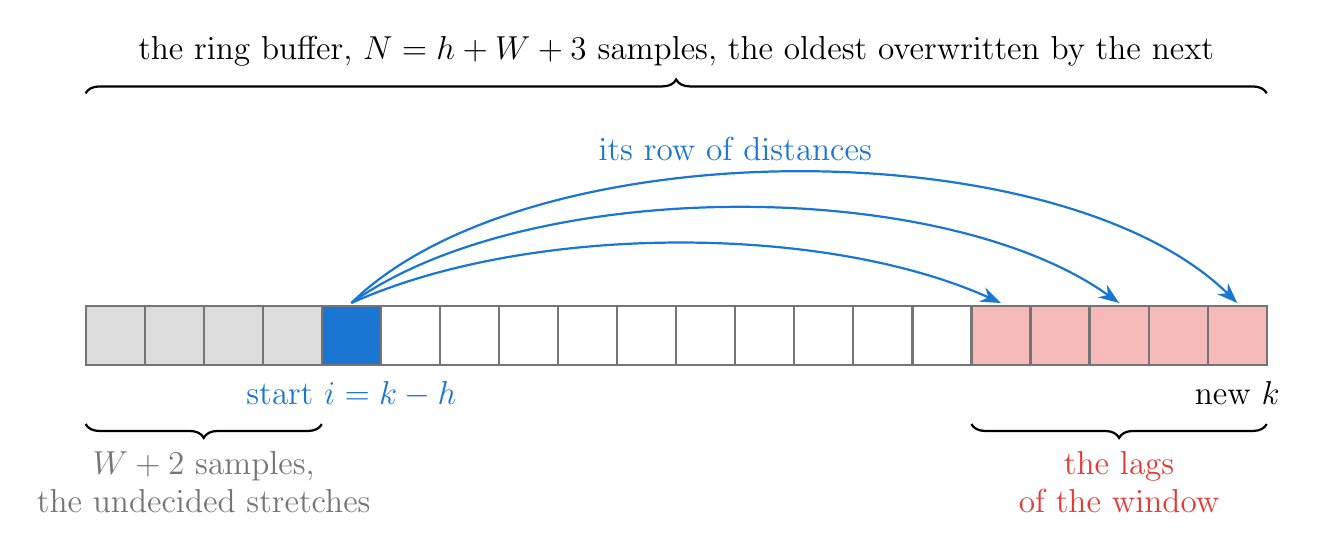
\begin{tikzpicture}[>={Stealth[length=2.6mm]}, every node/.style={font=\large}, x=0.75cm, y=0.75cm,
                    line width=0.8pt]
  % ---- the cells ----
  \foreach \k in {0,...,19} {
    \draw[cgrey, fill=white] (\k, 0) rectangle ++(1, 1);
  }
  \foreach \k in {0,...,3} { \draw[cgrey, fill=cgrey!25] (\k, 0) rectangle ++(1, 1); }
  \draw[cgrey, fill=cblue] (4, 0) rectangle ++(1, 1);
  \foreach \k in {15,...,19} { \draw[cgrey, fill=cred!35] (\k, 0) rectangle ++(1, 1); }

  % ---- the row of the start i, from it to three of the samples at its lags ----
  \draw[->, cblue] (4.5, 1.05) .. controls (7.5, 2.4) and (12.5, 2.4) .. (15.5, 1.05);
  \draw[->, cblue] (4.5, 1.05) .. controls (7.5, 3.2) and (14.5, 3.2) .. (17.5, 1.05);
  \draw[->, cblue] (4.5, 1.05) .. controls (7.5, 4.0) and (16.5, 4.0) .. (19.5, 1.05);
  \node[cblue] at (11.0, 3.65) {its row of distances};

  % ---- the labels under the cells ----
  \node[cblue, below] at (4.5, -0.1) {start $i = k - h$};
  \node[below] at (19.5, -0.1) {new $k$};
  \draw[decorate, decoration={brace, mirror, amplitude=5pt}] (0, -1.0) -- (4, -1.0)
      node[midway, below=6pt, cgrey, align=center] {$W + 2$ samples,\\ the undecided stretches};
  \draw[decorate, decoration={brace, mirror, amplitude=5pt}] (15, -1.0) -- (20, -1.0)
      node[midway, below=6pt, cred, align=center] {the lags\\ of the window};

  % ---- the whole buffer ----
  \draw[decorate, decoration={brace, amplitude=5pt}] (0, 4.6) -- (20, 4.6)
      node[midway, above=6pt] {the ring buffer, $N = h + W + 3$ samples, the oldest overwritten by the next};
\end{tikzpicture}
\end{document}
}
\caption{The ring buffer, drawn with $h = 15$ and $W = 2$. The new sample $k$ completes the row of the start $i = k - h$, its distances to the samples at the lags of the window (arrows). The $W + 2$ samples before $i$ hold the stretches of the candidates not yet decided.}
\label{fig:buffer}
\end{figure}

\begin{figure}[t]
\centering
\resizebox{0.9\textwidth}{!}{\documentclass[border=6pt]{standalone}
\usepackage{amsmath,amssymb}
\usepackage{xcolor}
\usepackage{tikz}
\usetikzlibrary{arrows.meta,backgrounds}
\definecolor{cblue}{HTML}{1976D2}
\definecolor{cred}{HTML}{E53935}
\definecolor{cpurple}{HTML}{5E35B1}
\definecolor{cgrey}{HTML}{757575}
\tikzset{every picture/.append style={show background rectangle,
    background rectangle/.style={fill=white}, inner frame sep=4pt}}
% The rows of one window, drawn with W = 2: the start down the page, the lag across. Three rows are
% stored, the older ones are discarded and keep only their candidates. A candidate is an entry of the
% middle row below the threshold and below its eight neighbours. A candidate within W of a smaller one
% is dropped. A candidate within W + 1 rows of the middle row is undecided, since the middle row may
% still bring a smaller one within W, and one further back is decided.
\begin{document}
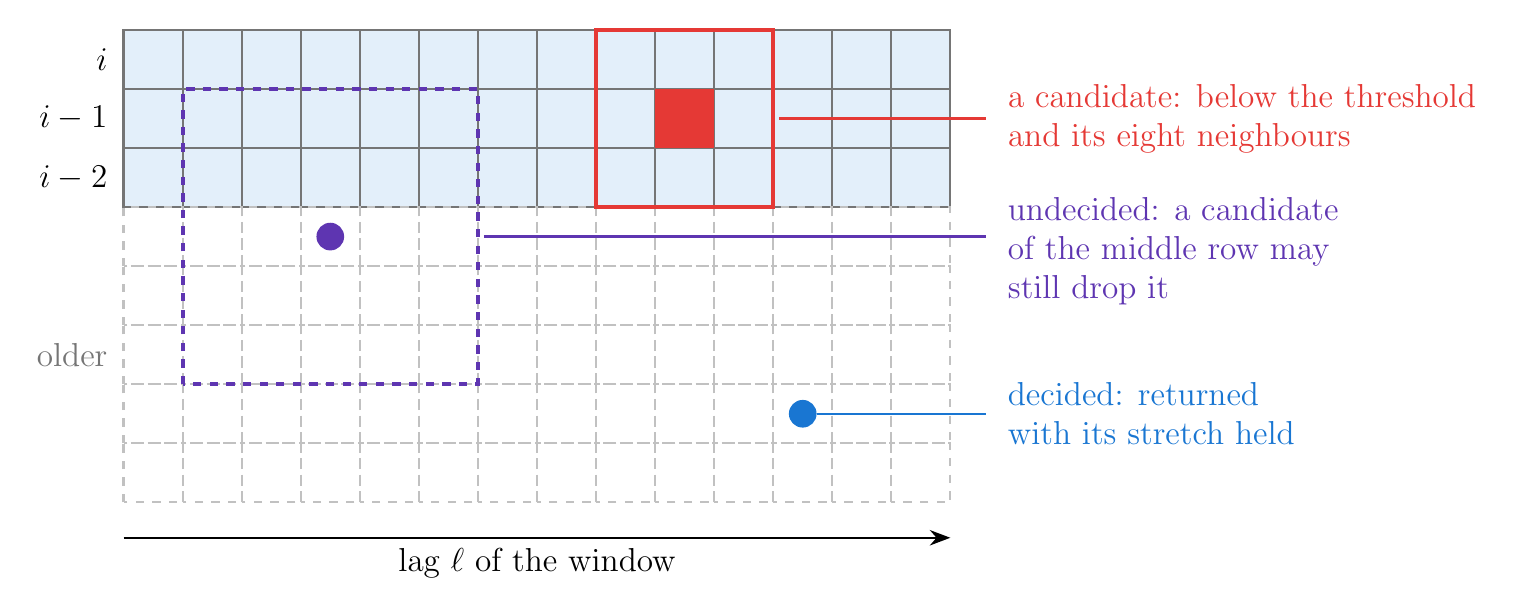
\begin{tikzpicture}[>={Stealth[length=2.6mm]}, every node/.style={font=\large}, x=0.75cm, y=0.75cm,
                    line width=0.8pt]
  % ---- the stored rows and the discarded ones ----
  \foreach \r in {0,...,7} {
    \foreach \c in {0,...,13} {
      \ifnum\r<3
        \draw[cgrey, fill=cblue!12] (\c, -\r) rectangle ++(1, 1);
      \else
        \draw[cgrey!45, dashed] (\c, -\r) rectangle ++(1, 1);
      \fi
    }
  }
  \node[left] at (-0.1, 0.5) {$i$};
  \node[left] at (-0.1, -0.5) {$i - 1$};
  \node[left] at (-0.1, -1.5) {$i - 2$};
  \node[left, cgrey] at (-0.1, -4.5) {older};

  % ---- the test of an entry of the middle row ----
  \draw[cred, line width=1.6pt] (8, -2) rectangle ++(3, 3);
  \fill[cred] (9, -1) rectangle ++(1, 1);

  % ---- an undecided candidate, with its square of side 2W ----
  \draw[cpurple, dashed, line width=1.4pt] (1, -5) rectangle ++(5, 5);
  \fill[cpurple] (3.5, -2.5) circle (5pt);

  % ---- a decided one ----
  \fill[cblue] (11.5, -5.5) circle (5pt);

  % ---- the labels, right of the rows ----
  \draw[cred, line width=0.8pt] (11.1, -0.5) -- (14.6, -0.5);
  \node[cred, right, align=left] at (14.8, -0.5) {a candidate: below the threshold\\ and its eight neighbours};
  \draw[cpurple, line width=0.8pt] (6.1, -2.5) -- (14.6, -2.5);
  \node[cpurple, right, align=left] at (14.8, -2.75) {undecided: a candidate\\ of the middle row may\\ still drop it};
  \draw[cblue, line width=0.8pt] (11.75, -5.5) -- (14.6, -5.5);
  \node[cblue, right, align=left] at (14.8, -5.5) {decided: returned\\ with its stretch held};

  % ---- the axis ----
  \draw[->] (0, -7.6) -- (14, -7.6) node[midway, below] {lag $\ell$ of the window};
\end{tikzpicture}
\end{document}
}
\caption{The rows of one window, drawn with $W = 2$, the start down the page and the lag across. Three rows are stored, and the older rows keep only their candidates. A candidate within $W + 1$ rows of the middle row is undecided, since a candidate of the middle row may still lie within $W$ of it. One further back is decided.}
\label{fig:rows}
\end{figure}

Two candidates are close if their starts differ by $W$ samples at most and their lags too, in any windows. A candidate is kept unless a close one comes before it in the order of the keys
\begin{equation}
(d,\ \text{start},\ \text{lag},\ \text{window}),
\label{eq:order}
\end{equation}
compared one after the other. Of two close candidates, the one of smaller distance is thus kept and the other is dropped, whatever their windows and their shifts. Two kept candidates are never close, since the later one in \eqref{eq:order} would be dropped. The last three keys break ties of distance. A tie arises where two windows overlap and one pair is a candidate of both, which the rule then keeps once, in the window of lower index. The rule depends on the candidates alone, not on the order in which they come. Figure~\ref{fig:search} shows what it removes on the Lorenz system.

A candidate of the start $s$ depends on the candidates of the starts $s - W$ to $s + W$. A later candidate starts at the middle row or after it, so these have all come once the middle row has reached $s + W + 1$. The sample $k$, whose middle row is $k - h - 1$, thus decides the candidates of the start
\begin{equation}
s = k - h - 2 - W,
\label{eq:decided}
\end{equation}
and returns those kept. A dropped candidate stays while a later decision needs it, that is while its start lies above $s - W$. The candidates of every window are decided in step with the longest one. A recurrence of a short window becomes final some $h$ samples after its stretch has come, and its stretch stays in the buffer until then.

The samples live in a ring buffer shared by all the windows, sample $k$ in slot $k \bmod N$. Its length follows from \eqref{eq:decided}. The stretch of a recurrence decided at the sample $k$ reaches from its start $k - h - 2 - W$ to at most $k$, and it must still be held. The buffer thus holds the samples $k - h - 2 - W$ to $k$, that is
\begin{equation}
N = h + W + 3 .
\label{eq:buffer}
\end{equation}
The next sample overwrites $k + 1 - N = k - h - 2 - W$, the start of the oldest stretch, which is thus held exactly until then. $W$ may exceed the width of a window and its lags. It only delays the decisions by \eqref{eq:decided} and lengthens the buffer by \eqref{eq:buffer}. With $W = 30/\Delta s = 300$ and a state of $34 \times 67$ complex coefficients, 36\,kB, the buffer takes 87\,MB for the bands up to 200 and 0.89\,GB for periods up to 2400.

The memory stays the same along a run of any length. The candidates held start within the $2W + 2$ rows from $s - W + 1$ to the middle row, and being minima below the threshold they are few. Their vector grows only when they outnumber all those held before. The recurrences decided at one sample all start at $s$ and are not close, so their lags differ by more than $W$, and there are at most $\lceil (h - \ell_{\rm lo} + 1)/(W + 1) \rceil$ of them, with $\ell_{\rm lo}$ the lowest lag. Their vector is given that capacity once.

Two windows that touch, $(T_{\rm lo}, T_1)$ and $(T_1, T_{\rm hi})$, share the lag $T_1/\Delta s$. It is the last lag of one and the first of the other, so a minimum there is a candidate of neither. Windows that overlap by two lags or more find it, and the rule of the closest keeps it once.

\begin{figure}[t]
\centering
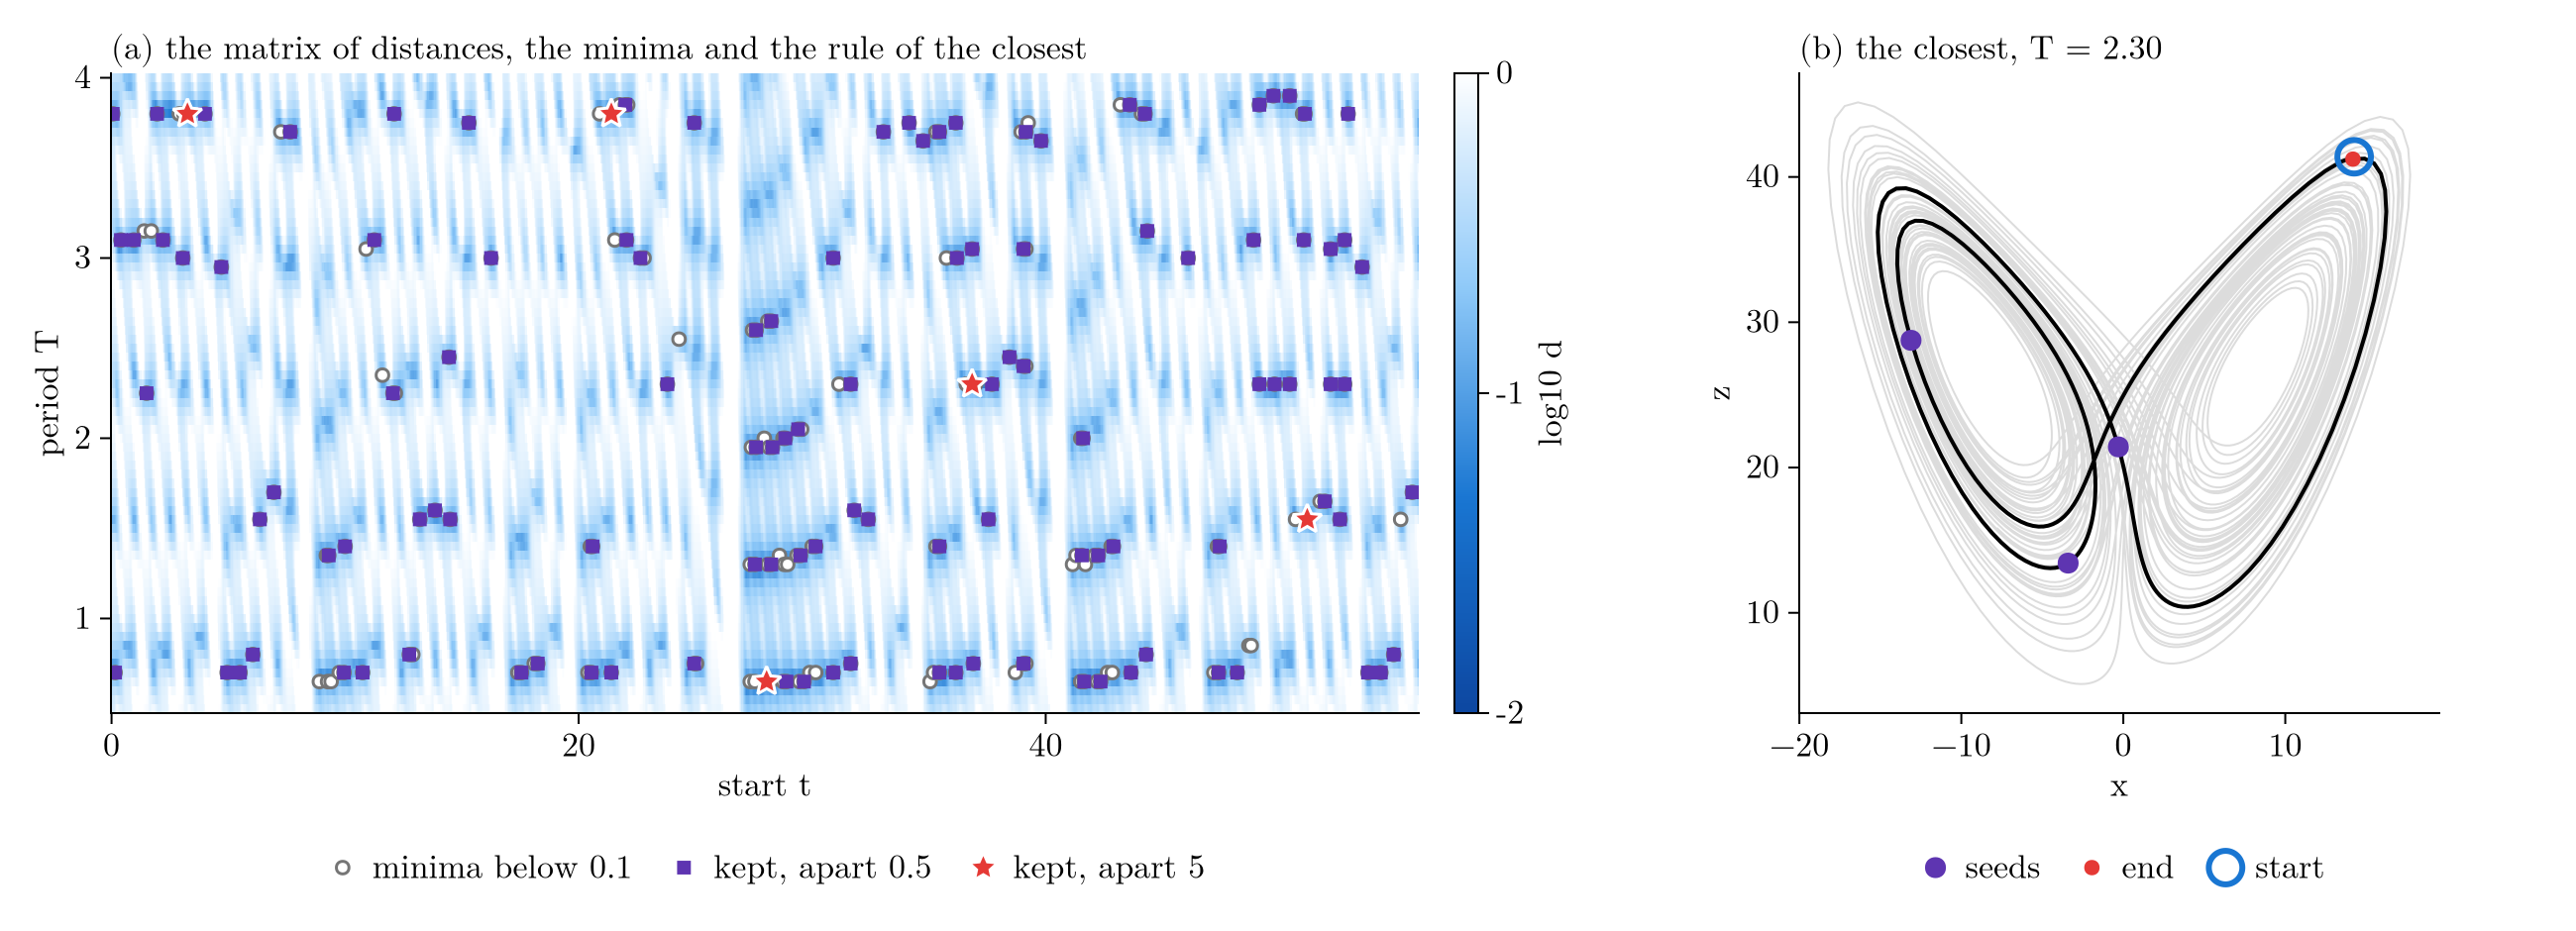
\includegraphics[width=\textwidth]{../examples/lorenz/search.png}
\caption{The search on the Lorenz system at $\sigma = 10$, $\rho = 28$, $\beta = 8/3$, sampled every $\Delta s = 0.05$ by five steps of the classical Runge--Kutta scheme, for the periods from 0.5 to 4 below $d_p = 0.1$, with the distance $\|\bu(t + T) - \bu(t)\|/\|\bu(t)\|$. (a) The matrix of distances of the first 60 time units, its minima below $d_p$ (open circles), and those kept by the rule of the closest with $W = 0.5$ (squares) and $W = 5$ (stars), half a Lyapunov time and some four. (b) The closest recurrence of the wide rule over $10^4$ time units in the plane $(x, z)$, with the seeds of four segments (section~\ref{sec:seeds}). From \code{examples/lorenz/search.jl}.}
\label{fig:search}
\end{figure}

\section{Several symmetries}
\label{sec:shifts}

The distance \eqref{eq:distance} is minimised over all the symmetries at once, and the search sees the minimum alone. A near recurrence is thus a local minimum over $(t, T)$ of the distance already minimised over the symmetries, and it carries the shifts of its own pair, $(\sigma, s_y)$ for Kolmogorov flow. Its neighbours in the rows may reach their minima at other shifts. The rule of the closest compares distances alone, so of two close minima with different discrete shifts the smaller is kept and the other is dropped.

The Lorenz system gives a small model. It does not change under the rotation $R(x, y, z) = (-x, -y, z)$ by $\pi$ about the $z$ axis, a discrete symmetry, and the distance up to it is
\begin{equation}
d = \frac{\min\big(\|b - a\|,\ \|R b - a\|\big)}{\|a\|},
\end{equation}
returned with the rotations $r \in \{0, 1\}$ of $b$ that reach it. A recurrence with $r = 1$ closes after the rotation, as the two halves of a symmetric orbit do (figure~\ref{fig:symmetry}). The translation along $y$ of Kolmogorov flow is such a discrete shift, and the shift along $x$ a continuous one.

\begin{figure}[t]
\centering
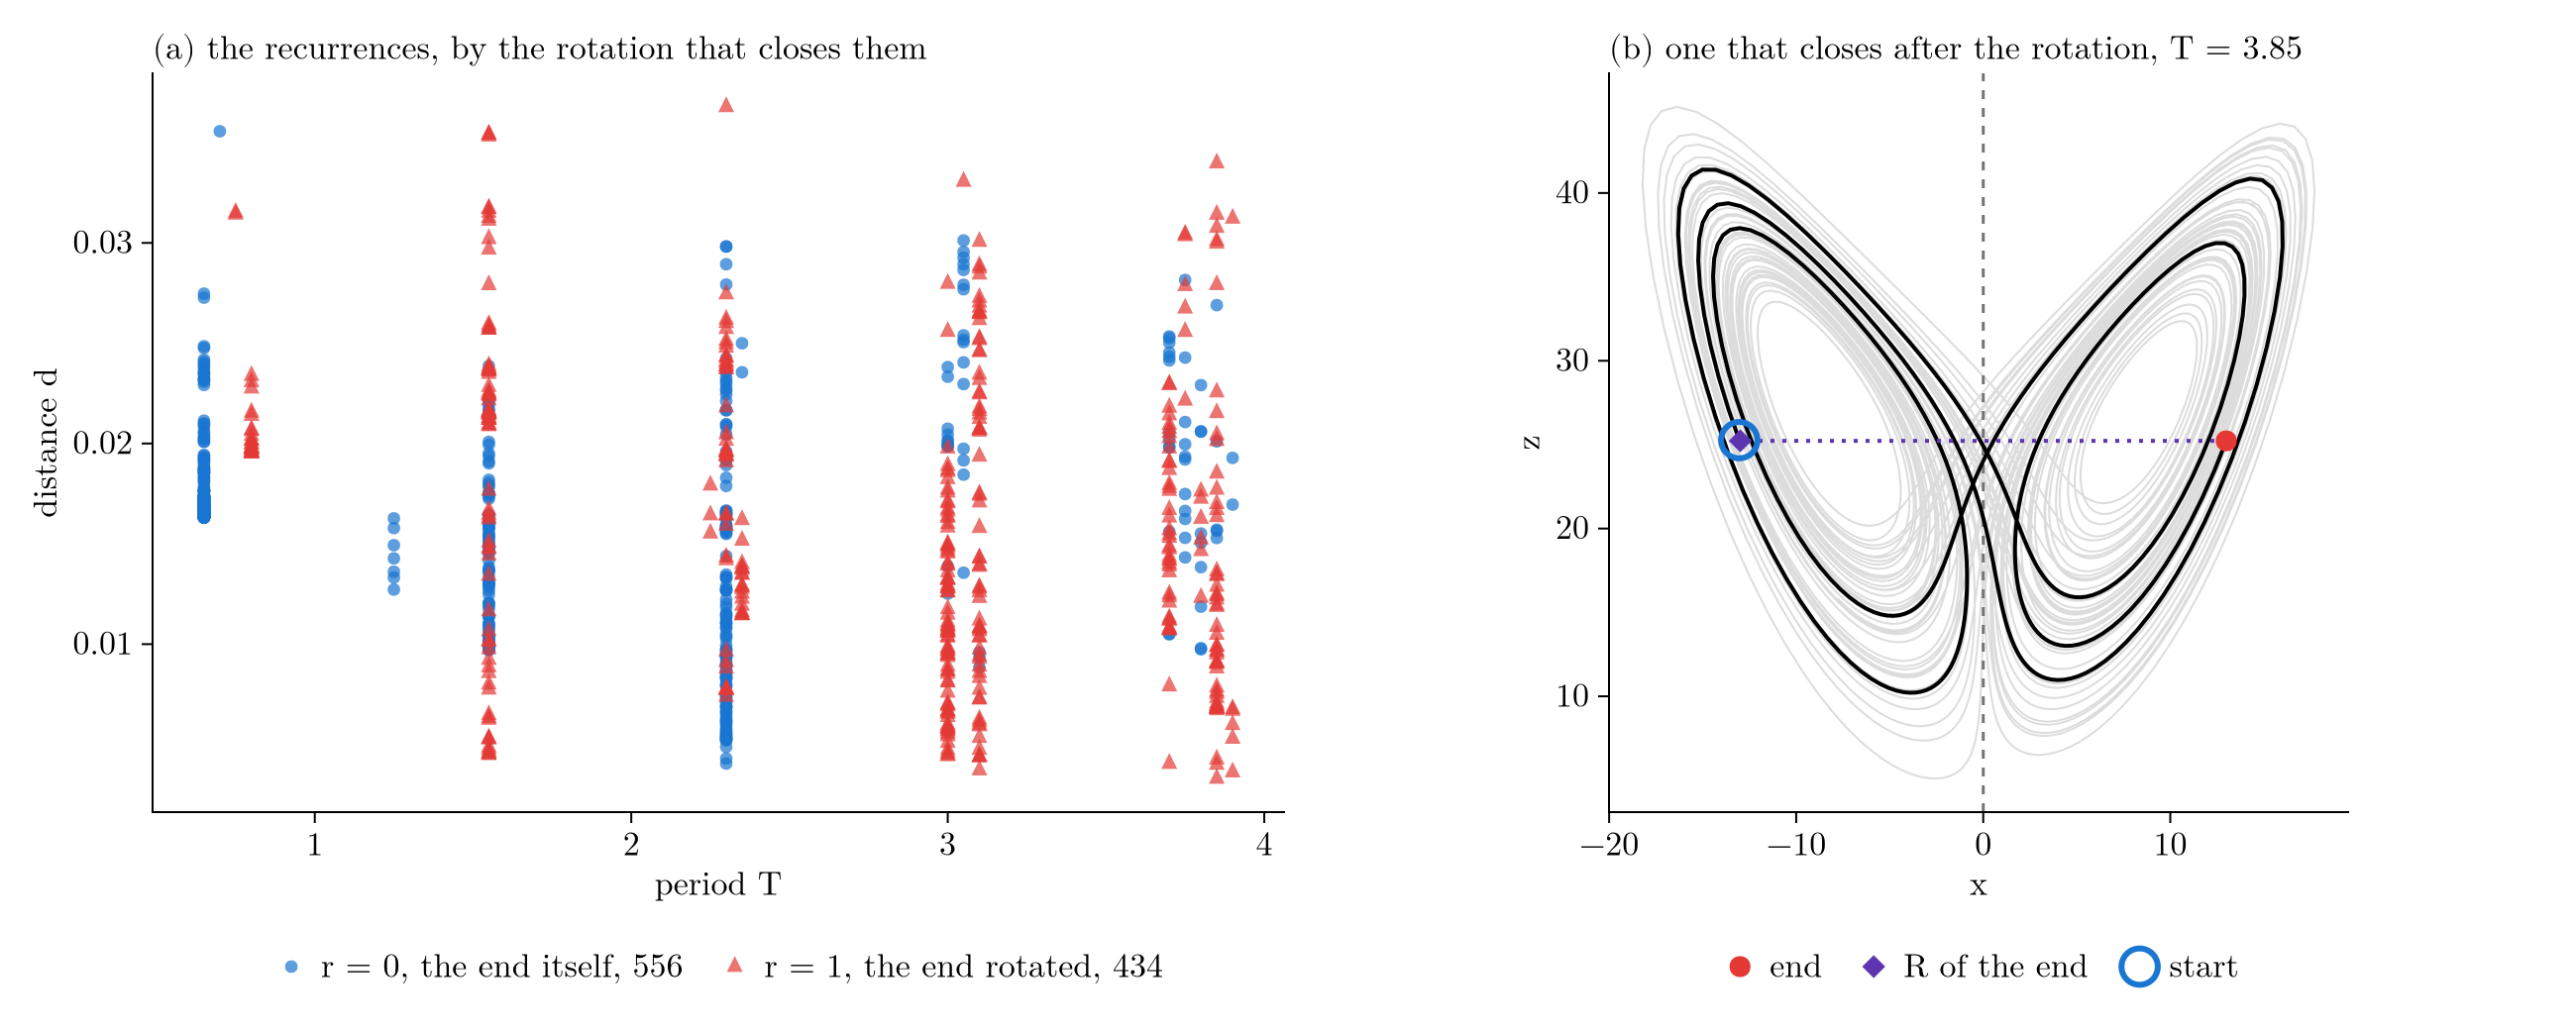
\includegraphics[width=\textwidth]{../examples/lorenz/symmetry.png}
\caption{The search on the Lorenz system up to the rotation $R$, with $W = 5$, over $10^4$ time units, otherwise as figure~\ref{fig:search}. (a) The recurrences, by the rotation that closes them. (b) The closest of those that close after the rotation, in the plane $(x, z)$, where $R$ is the mirror $x \to -x$ (dashed). Its end, rotated, lies near its start. From \code{examples/lorenz/symmetry.jl}.}
\label{fig:symmetry}
\end{figure}

\section{The bound by an invariant}
\label{sec:bound}

Most pairs lie far above $d_p$, and a cheaper quantity can tell them apart before the minimum over the shifts. An invariant is a real array $v(\bu)$ with three properties,
\begin{equation}
v(\mathcal{S}\bu) = v(\bu) \ \text{for every symmetry}, \qquad \|v(a) - v(b)\| \le \|a - b\|, \qquad \|v(a)\| = \|a\| .
\label{eq:invariant}
\end{equation}
The symmetries leave it unchanged, it does not stretch distances, and it keeps the norm. For every symmetry $\mathcal{S}$ the first two give
\begin{equation}
\|v(b) - v(a)\| = \|v(\mathcal{S} b) - v(a)\| \le \|\mathcal{S} b - a\| ,
\end{equation}
so $\|v(b) - v(a)\|$ is at most the minimum over $\mathcal{S}$. Dividing by $\|v(a)\| = \|a\|$, the third property, gives the bound
\begin{equation}
\beta(a, b) = \frac{\|v(b) - v(a)\|}{\|v(a)\|} \le d(a, b) .
\label{eq:bound}
\end{equation}
The package normalises $\beta$ by the norm of the invariant of the start, as $d$ is normalised by the norm of the start, so \eqref{eq:bound} holds when the user's $v$ keeps the norm.

For the rotation of the Lorenz system, $v = (\sqrt{x^2 + y^2},\ z)$. The rotation changes the signs of $x$ and $y$ and leaves $\sqrt{x^2 + y^2}$ alone. By the reverse triangle inequality $\big|\,\|(x_b, y_b)\| - \|(x_a, y_a)\|\,\big| \le \|(x_b, y_b) - (x_a, y_a)\|$, so $v$ does not stretch distances, and $\|v\|^2 = x^2 + y^2 + z^2$. For Kolmogorov flow, $v$ holds the moduli $\sqrt{w_j}\,|\hat\omega_{jk}|$. The shift and the translation change the phases of the coefficients alone, so the moduli do not change. Mode by mode $\big||b_{jk}| - |a_{jk}|\big| \le |b_{jk} - a_{jk}|$, and the sum over the modes, with the weights, gives the other two properties.

A pair with $\beta \ge d_p$ is not compared in full, and its entry of the row holds $\beta$. The candidates stay those of the distances alone. Such an entry is at or above $d_p$, as its distance is by \eqref{eq:bound}, so it is no candidate. A candidate lies below $d_p$, so it lies below such a neighbour, as it lies below its distance. Figure~\ref{fig:invariant} draws $\beta$ against $d$ on the Lorenz system. The bound costs one pass over the invariants. In the searches of Kolmogorov flow at $p = 10^{-6}$ of table~\ref{tab:cost}, fewer than eight pairs in a thousand passed it, and a pair cost $1.2\,\mu$s instead of $11.6\,\mu$s on an EPYC 7502. Figure~\ref{fig:kolmogorov} draws the bound against the distance for Kolmogorov flow. Over a stream of 2000 time units, for the windows 19 to 21 and 95 to 105 at $d_p = 0.118$, the bound passed 139 of $2.3 \times 10^6$ pairs, and on one core of a laptop a bound cost $1.4\,\mu$s against $6.7\,\mu$s for a distance. No pair of the sample lies below $d_p$, and the stream found no recurrence, as the rates of figure~\ref{fig:numbers} predict, fewer than one per $10^5$ time units in these bands at $p = 10^{-6}$.

\begin{figure}[t]
\centering
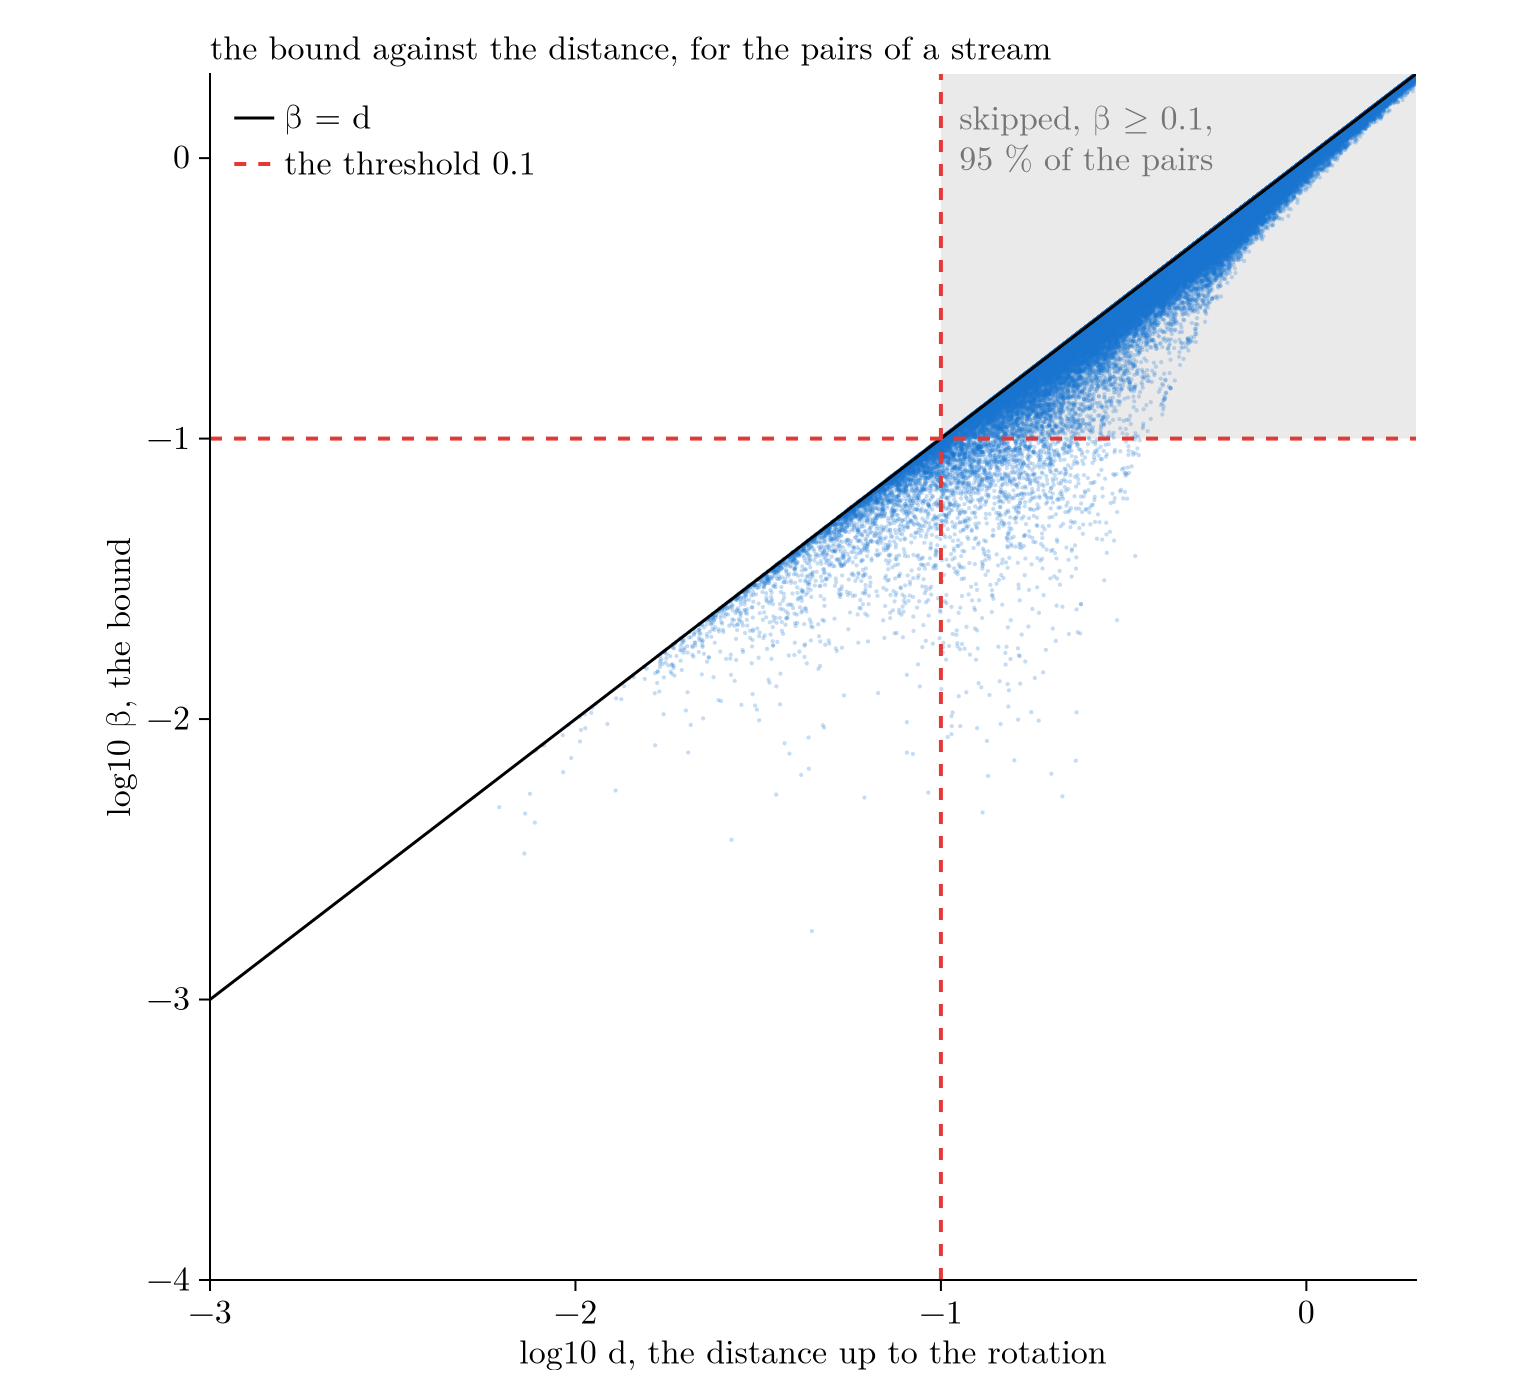
\includegraphics[width=0.55\textwidth]{../examples/lorenz/invariant.png}
\caption{The bound $\beta$ against the distance $d$ up to the rotation, for the pairs of every tenth start of 1000 time units of the Lorenz system at the lags of the window from 0.5 to 4. All lie below the diagonal. The pairs with $\beta \ge 0.1$ (shaded) are not compared in full, the fraction given over $10^4$ time units. From \code{examples/lorenz/invariant.jl}.}
\label{fig:invariant}
\end{figure}

\begin{figure}[t]
\centering
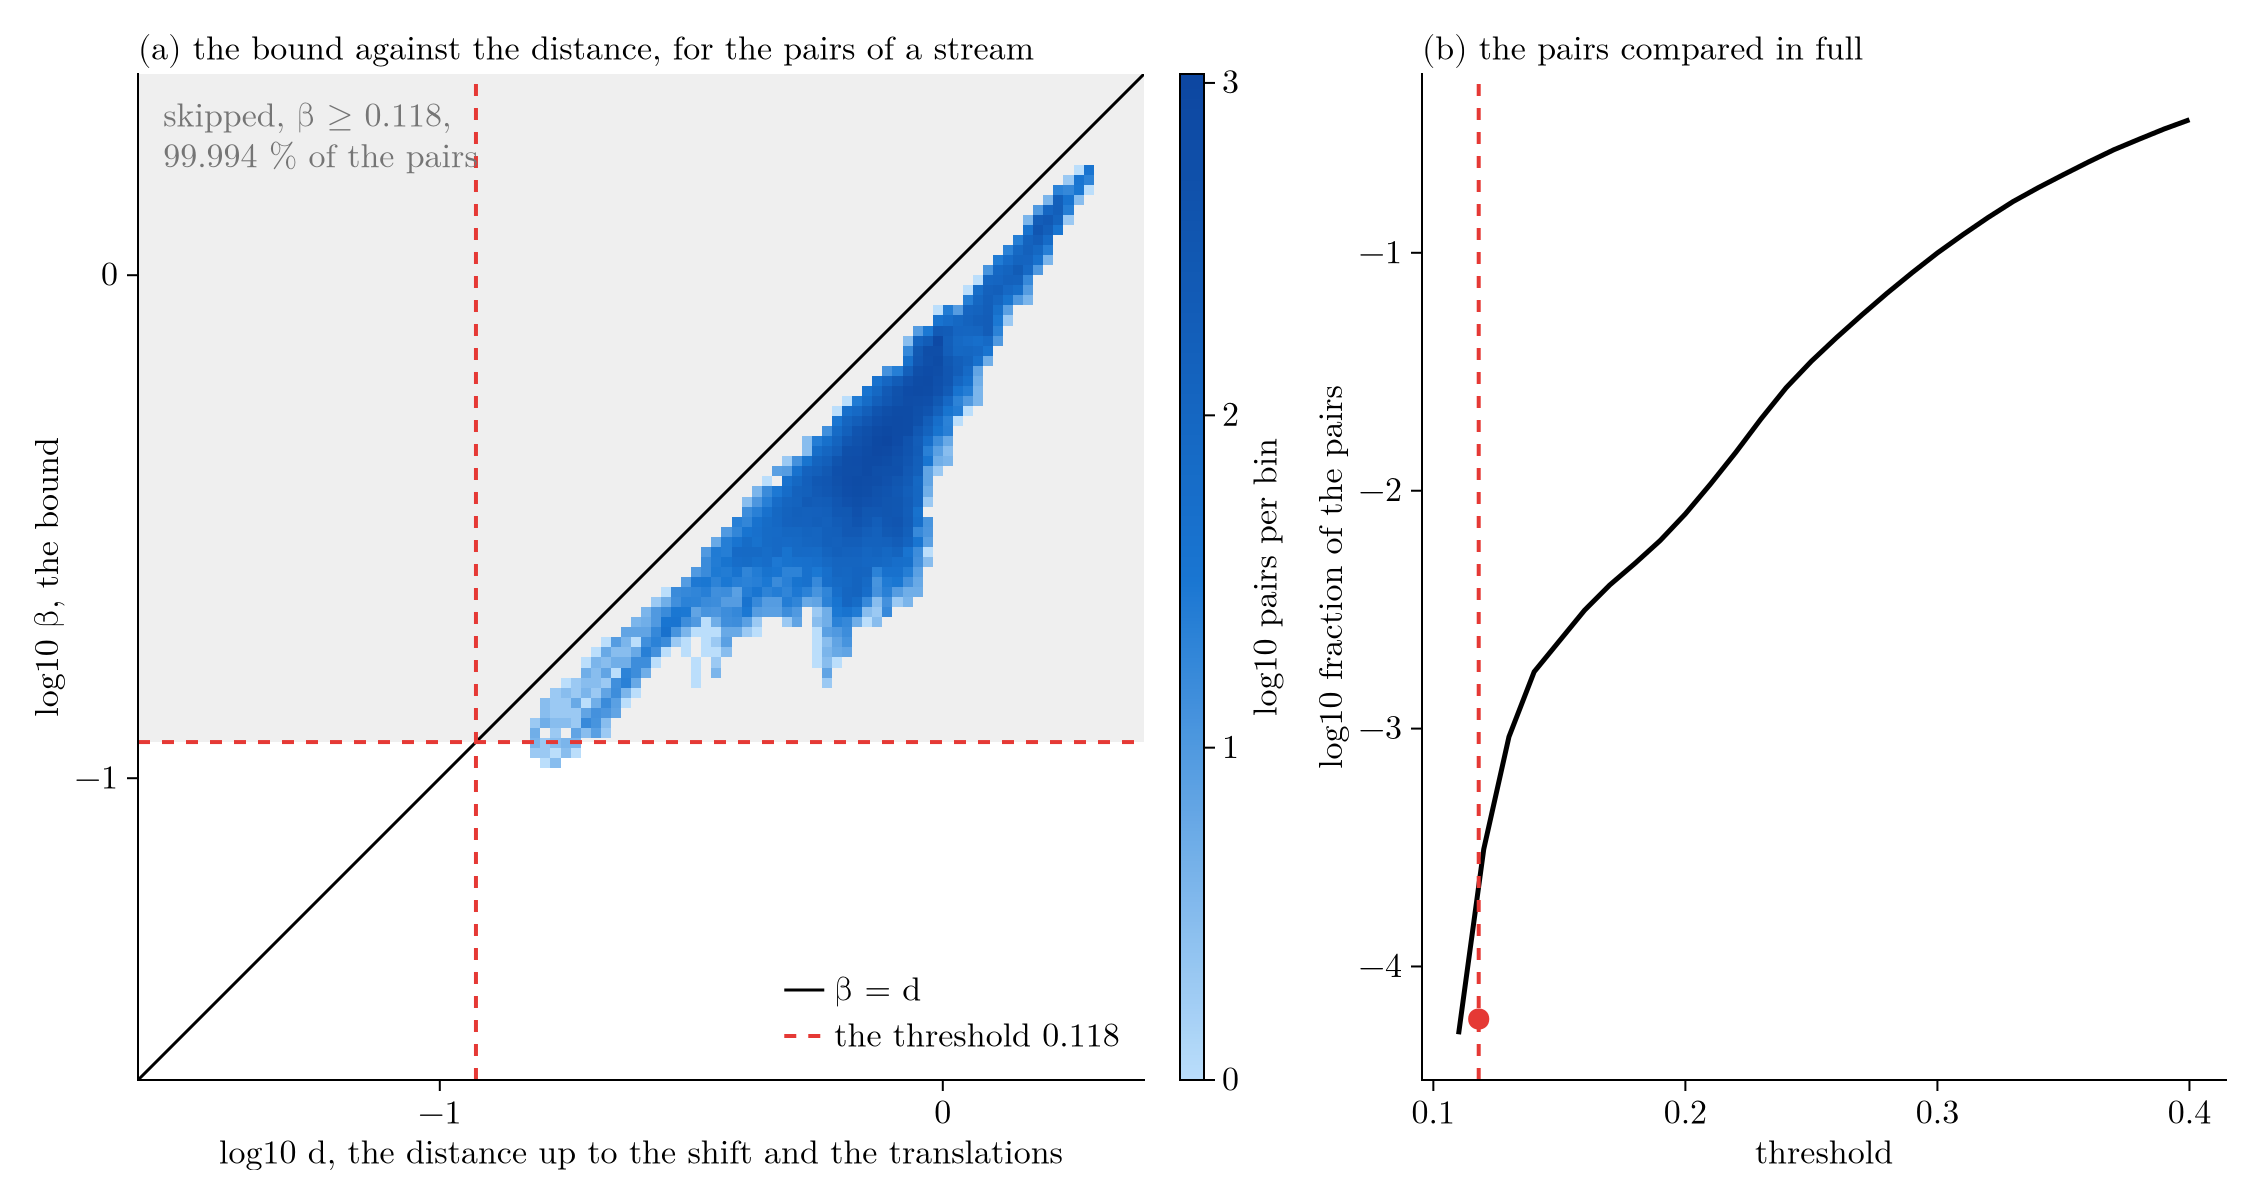
\includegraphics[width=\textwidth]{../examples/kolmogorov/bound.png}
\caption{The bound by the moduli on Kolmogorov flow at $Re = 40$, sampled every 0.1, for the windows of periods 19 to 21 and 95 to 105, with $d_p = 0.118$. (a) The density of the pairs of every fifth start of 500 time units over the bound and the distance up to the shift and the translations. All lie below the diagonal, and those above the horizontal line (shaded) are not compared in full, the fraction given over a stream of 2000 time units. (b) The fraction of the pairs compared in full against the threshold, the stream at 0.118 marked. From \code{examples/kolmogorov/bound.jl}.}
\label{fig:kolmogorov}
\end{figure}

\section{The probability of a distance}
\label{sec:probability}

The rows hold the distance of every pair at the lags of the windows, so the search can measure $C$ as it goes. Each window counts the pairs that it compares, $N_w$, and keeps a histogram of $\log_{10} d$ for the distances below its threshold. Bin $j$ holds
\begin{equation}
e_j \le \log_{10} d < e_{j+1}, \qquad e_j = -2 + (j - 1)/100,
\end{equation}
and the first bin the distances below $10^{-1.99}$ as well, up to the bin of the threshold. With the bound, a pair with $\beta \ge d_p$ counts in $N_w$ but is not binned. Every pair with $d < d_p$ has $\beta \le d < d_p$ by \eqref{eq:bound}, so it is compared in full and binned. The histogram below the threshold is thus the same with the bound or without it.

At an edge $e_j$ the pairs closer than $10^{e_j}$ are those of the bins below $j$. With $n_{wj}$ the count of bin $j$ of window $w$,
\begin{equation}
C\big(10^{e_j}\big) = \frac{\sum_w \sum_{i < j} n_{wi}}{\sum_w N_w}, \qquad 10^{e_j} \le \min_w d_{p,w},
\label{eq:probability}
\end{equation}
exactly. Between two edges $C$ is known to the edge below, a distance $10^{0.01}$, or 2.3 per cent, smaller at most. Several runs with the same thresholds add their counts bin by bin and their pairs, and \eqref{eq:probability} holds for the sums. A pair at a lag of two windows counts in both. Figure~\ref{fig:probability} draws $C$ of the Lorenz system and the distances of three probabilities.

\begin{figure}[t]
\centering
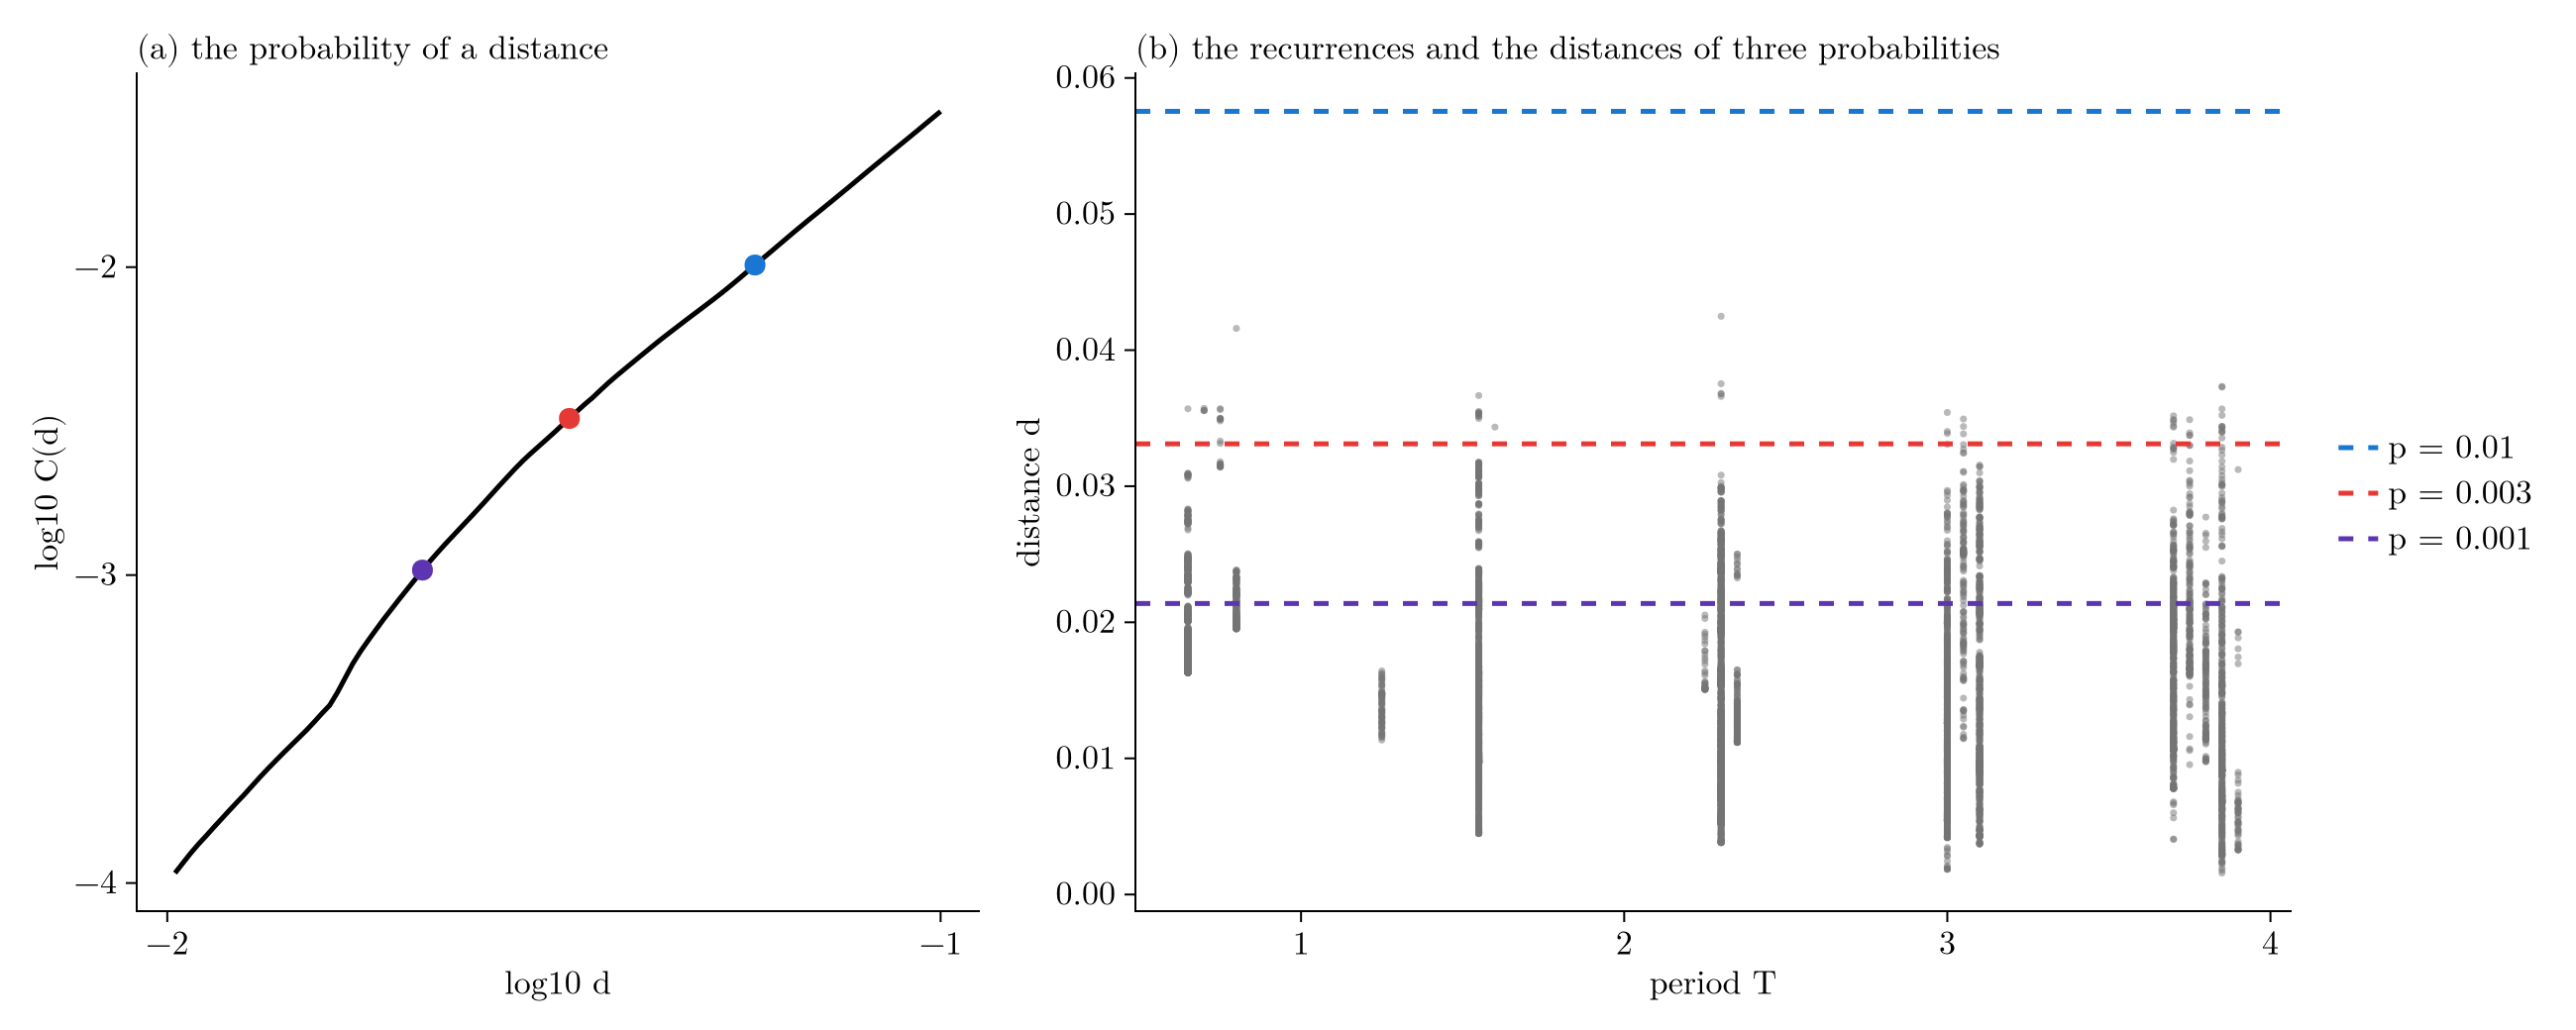
\includegraphics[width=\textwidth]{../examples/lorenz/probability.png}
\caption{The probability of a distance on the Lorenz system up to the rotation, over $10^5$ time units, otherwise as figure~\ref{fig:symmetry}. (a) The fraction $C(d)$ of the pairs closer than $d$, from the histogram. (b) The distance against the period of the recurrences, with the distances $d_p$ where $C$ reaches three probabilities. From \code{examples/lorenz/probability.jl}.}
\label{fig:probability}
\end{figure}

\section{The seeds of a search}
\label{sec:seeds}

A recurrence is the first guess of a search for a periodic orbit by multiple shooting. The search cuts the stretch into $m$ segments of length $\tau$, with the shooting points $\bu_1, \dots, \bu_m$. Its first residual has the interior junctions $\varphi_\tau(\bu_i) - \bu_{i+1}$ and the closing junction $\mathcal{S}\varphi_\tau(\bu_m) - \bu_1$. Let the shooting points be samples of the simulation, and let each segment repeat the steps that led from its point to the next. Each interior junction then vanishes, and the closing junction is $\mathcal{S}\bu(t + T) - \bu(t)$, with the shifts of the recurrence, so
\begin{equation}
\|\mathbf{F}_0\| = d\,\|\bu(t)\| .
\end{equation}
The search then starts from the recurrence and nothing else.

The start alone does not do. An integration gives back the simulation bit for bit only with the same floating-point operations, the same steps and the same FFT plan. A search on a GPU differs from the simulation on a CPU at the rounding, $10^{-15}$. The difference grows at $\lambda_1 = 0.13$ and reaches $d \approx 0.15$ after $\ln(1.5 \times 10^{14})/0.13 \approx 250$ time units. A long stretch rebuilt from its start on another device is thus another trajectory.

The shooting points are therefore samples, and every segment spans whole samples. For $m$ segments of a lag $\ell$ the offsets from the start are
\begin{equation}
o_j = \mathrm{round}\big((j - 1)\,\ell/m\big), \qquad j = 1, \dots, m + 1,
\label{eq:offsets}
\end{equation}
so that $o_1 = 0$ and $o_{m+1} = \ell$. Consecutive values $(j - 1)\ell/m$ differ by $\ell/m$, and rounding moves each by half a sample at most. A segment thus spans a whole number of samples between $\ell/m - 1$ and $\ell/m + 1$, that is $\ell/m$ when it is whole, and its floor or ceiling otherwise. With $\ell = 10$ and $m = 4$ the offsets are 0, 2, 5, 8 and 10, the values 2.5 and 7.5 rounded to the even neighbour.

For Kolmogorov flow the propagator of the searches checks this. From shooting points at the samples, on seven guesses on the CPU and on a GPU, the closing junction equals $d$ to $2 \times 10^{-13}$ of $d$ and the interior junctions miss by $2 \times 10^{-15}$ to $9 \times 10^{-13}$ of the norm. Shooting points between two samples, a sample advanced with a last step shorter than $\Delta t$, start their segments between two steps of the simulation. Their junctions then miss by the error of the time steps, up to $2 \times 10^{-7}$ of the norm at $\tau \approx 5$ and 10. A guess of $m$ segments takes $m + 1$ states, $36\,\mathrm{kB} \times (m + 1)$.

\section{The interface}

The package holds the loop of section~\ref{sec:stream} and nothing else. What knows the system stays with the user, the time stepping, the distance with its symmetries, and the writing of files. The search of the long simulations of Kolmogorov flow reads
\begin{Verbatim}
import NearRecurrences
import BatchedKolmogorovFlow
import Random
import Serialization

n, m, Re, kf = 33, 49, 40.0, 4
G = BatchedKolmogorovFlow.NonlinearPropagator(n, m, Re, kf; B=1, dt=0.01)

x  = Random.randn!(BatchedKolmogorovFlow.FTFields(n, 1))    # a smooth random field
x .= x ./ (1 .+ x.j.^2 .+ x.k.^2)
BatchedKolmogorovFlow.apply_symmetry!(x)
G(x, 500.0)                                                  # the transient

R = NearRecurrences.Recurrences(x, BatchedKolmogorovFlow.Distance(n, kf);  # (d, sigma, sy)
                                spacing   = 0.1,
                                windows   = [(19, 21), (173, 245), (1414, 2400)],
                                threshold = 0.118,
                                apart     = 30.0,
                                invariant = BatchedKolmogorovFlow.moduli)

for k in 1:10^7
    G(x, 0.1)                                                # one sample, ten steps
    for r in push!(R, x)
        g = NearRecurrences.seeds(R, r, max(1, round(Int, r.T/10)))
        Serialization.serialize("r$(r.start)-$(r.lag).jls", (r, g))
    end
end
rest = NearRecurrences.finish!(R)
NearRecurrences.probability(R, 0.091)
\end{Verbatim}
\code{Distance(n, kf)} returns $(d, \sigma, s_y)$ by \eqref{eq:poly}, minimised over the shift and the four translations, and \code{moduli} the invariant of section~\ref{sec:bound}. A recurrence \code{r} is the named tuple \code{(t, T, d, shifts, window, start, lag)}, with the shifts $(\sigma, s_y)$ after the distance. \code{seeds} returns the $m + 1$ states at the offsets \eqref{eq:offsets}, copies of the samples, and the offsets. The rule of the closest keeps one of the minima within 30 time units, about four Lyapunov times, since closer ones repeat one guess.

Five choices shape the interface. First, one buffer over the longest lag serves all the windows. The trajectory is integrated once whatever the number of windows, and every stretch is held. The price is $N$ states in memory by \eqref{eq:buffer}. A stream per window would hold only the width of its window, but each would integrate the trajectory again and none would hold a stretch.

Second, the loop belongs to the user. \code{push!} returns the recurrences that the sample makes final, and their stretches are held until the next \code{push!}, by \eqref{eq:buffer}. The seeds are then copied in place, from the buffer, and only those asked for. A callback would do the same with one more function to pass, and an iterator over the recurrences would have to copy every stretch, up to 24\,000 states at $T = 2400$. The vector returned is reused by the next \code{push!}, so a run allocates nothing after the start but the growth of the candidates to a new largest number.

Third, the rule of the closest acts across the windows. The long windows of the flow touch, and two minima on either side of a common edge repeat one guess as much as two minima within a window do. One list of candidates for all the windows, decided in step with the longest one, does this at no cost in memory, since the buffer \eqref{eq:buffer} is set by the longest window anyway.

Fourth, the distance returns its shifts with it, and the rows hold distances only. A recurrence takes its shifts from one more call of the distance when it is kept, which is rare.

Fifth, the bound comes from an invariant, a keyword. Any invariant with \eqref{eq:invariant} serves, and a test can check $\beta \le d$ on every pair. A distance that stops early once it exceeds $d_p$ would be more general but would tie the user's function to the search.

\section{The numbers}

The recurrences of $3.2 \times 10^7$ time units of simulation of Kolmogorov flow, searched in the bands 20 to 2000 with the shift along $x$ alone, are 7128 below $p = 10^{-5}$, from 290 in the band 30 to 1375 in the band 200 (figure~\ref{fig:numbers}a). Simulations of $5 \times 10^4$ to $10^5$ time units with the translations along $y$ as well add windows of periods up to $10^4$. These searches kept the smaller of two minima within 10 time units in one band.

\begin{figure}[t]
\centering
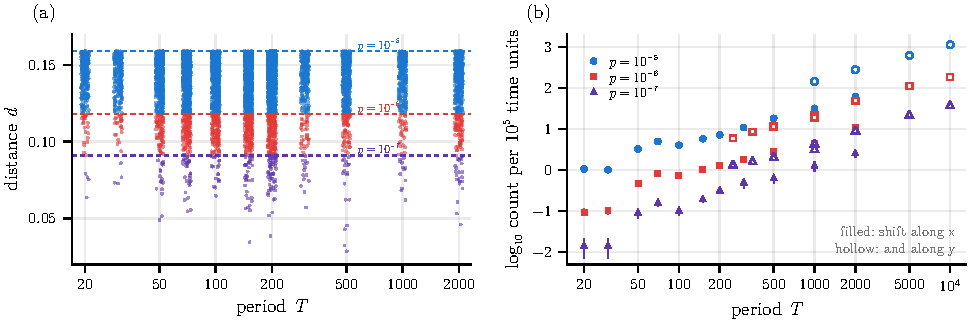
\includegraphics[width=\textwidth]{figures/counts.pdf}
\caption{The recurrences of Kolmogorov flow. (a) The distance against the period of the 7128 recurrences found with the shift along $x$ alone, with the distances $d_p$ of three probabilities. (b) The recurrences per $10^5$ time units in a band $T \pm 5$ per cent below $d_p$, with the shift along $x$ alone (filled) and with the translations along $y$ as well (hollow, the windows scaled to $\pm 5$ per cent about their middle). Bars, $\pm\sqrt{n}$ of a count $n$. From \code{fig\_counts.jl}.}
\label{fig:numbers}
\end{figure}

Two rules describe the counts (figure~\ref{fig:numbers}b). The count in a band grows as $T$, about $0.035\,T$ per $10^5$ time units at $p = 10^{-5}$ from $T = 100$ on. The band is $0.1\,T$ wide, and a unit of width collects nearly the same number, a fifth less at $T = 10^4$ than at $T = 100$. The count also falls with the distance as $d^{\mu}$, with $\mu = 6.0$ by maximum likelihood (7.4 in the bands 20 and 30), more slowly than $C \propto d^{7\text{--}8}$. The reason is that a recurrence is a minimum. Near a minimum of depth $d_0$, $d^2 - d_0^2$ grows as a quadratic form in the offsets of $t$ and $T$, so the pairs closer than $d$ fill an area of the plane $(t, T)$ proportional to $d^2 - d_0^2$. Summing over the minima, whose number below $d$ grows as $d^{\mu}$, adds two powers, and $C \propto d^{\mu + 2}$. Hence one recurrence in six below $p = 10^{-5}$ lies below $10^{-6}$, and one in thirty below $10^{-7}$, not one in 10 and 100. The four translations along $y$ are equally frequent, each a quarter of the recurrences found with them, so with them the count is four times larger (3.97).

\begin{table}[t]
\centering
\caption{The cost of a time unit of simulation of Kolmogorov flow on one core, in seconds, for the integration and for the distances of the windows, the pairs compared per sample and the ring buffer of \eqref{eq:buffer}, with $W = 300$ and the moduli held with the samples when the bound is used. Medians over the runs.}
\label{tab:cost}
\small
\begin{tabular}{l l l r r r r}
\toprule
periods & bound & CPU & integration & distances & pairs per sample & buffer \\
\midrule
20--200 & no & EPYC 9655 & 0.066 & 0.049 & 627 & 87\,MB \\
300--2000 & no & EPYC 7502 & 0.106 & 0.44 & 3804 & 0.78\,GB \\
19--245 & yes & EPYC 7502 & 0.104 & 0.014 & 1147 & 0.15\,GB \\
19--2400 & yes & EPYC 7502 & 0.104 & 0.083 & 22\,701 & 1.3\,GB \\
\bottomrule
\end{tabular}
\end{table}

The integration costs 0.066\,s per time unit on an EPYC 9655 and 0.106\,s on an EPYC 7502 (table~\ref{tab:cost}). A band $T \pm 5$ per cent costs $10\,(T + 1)$ distances per time unit, so the distances pass the integration once the windows hold $0.066/(10 \times 7.8\,\mu\mathrm{s}) \approx 850$ lags, as the bands 300 to 2000 do, where they take four fifths of the time. The bound \eqref{eq:bound} raises this to about 9000 lags. With it, the windows up to 245 spend an eighth of the time on the distances, and those up to 2400, with 22\,701 lags, under half. The cost per pair falls with the number of lags, from $1.2\,\mu$s at 1147 lags to $0.37\,\mu$s at 22\,701, since the moduli of a sample are computed once for all its pairs.

\section*{Reference}

G. J. Chandler and R. R. Kerswell, Invariant recurrent solutions embedded in a turbulent two-dimensional Kolmogorov flow, \emph{J. Fluid Mech.} \textbf{722}, 554--595 (2013).

\end{document}
